\chapter{Evaluation}\label{chap:evaluation}

Neither persistent base nodes nor snapshotting lead to direct performance
benefits for Soup. Instead, they both come with a wide range of features and
improvements in other areas, helping Soup make a significant leap towards being
a production-ready database system. Moving the base node state to durable
storage lets Soup operate on datasets larger than its memory size, while
reducing the overall memory usage of the system. It improves the system's
overall recovery capabilities---a necessity if Soup is ever going to be usable
for long running applications. Snapshotting takes this a step further, and
removes the performance penalty Soup sees while its partial states are brought
back to the state they were prior to a fatal failure.

Regardless, Soup's performance when faced with a large amount of concurrent
requests is still one of its main contributions. While a certain reduction in
throughput and latency might be inevitable, it is crucial that this penalty
remains as insignificant as possible. This chapter first investigates the
effects \code{PersistentState} has on performance, followed by a look at the
recovery benefits from both \code{PersistentState} and snapshotting.

\newpage

\section{Write-performance}

Only a small subset of reads propagate all the way to the base nodes. Instead,
they are served by partially materialized nodes further down the graph, avoiding
the need for expensive computations on each read. This is not the case with
writes. Every update that reaches Soup needs to be fully persisted to durable
storage before a write acknowledgment can be sent. With persistent base nodes,
that involves materializing the updates into \code{PersistentState}. With
packets being processed synchronously at each domain, even the smallest increase
in write latency at the base nodes could have disastrous effects for the overall
write throughput of the system.

The \code{vote} benchmark described in section~\ref{sec:vote} is used to measure
write-performance. While it is normally a mixed-load benchmark where clients
both write new votes and read the existing vote counts of articles, we will run
\code{vote} with a pure write-load, removing reads altogether. Since we are
measuring the impact of writing to durable storage, Soup will run without
sharding, resulting in a single domain writing new votes to
\code{PersistentState}. The database is pre-populated with 100K articles and the
inserted votes are uniformly distributed across the existing articles.

Soup can be run both in a local and distributed fashion, and \code{vote}
supports both. Writing to durable storage is a penalty fixed per machine
however, and benchmarking the horizontal scalability makes little sense.
Instead, we will use the \textit{local} \code{vote} benchmark, where both the
clients and the Soup workers run on the same machine.

\begin{figure}[H]
  \centering
  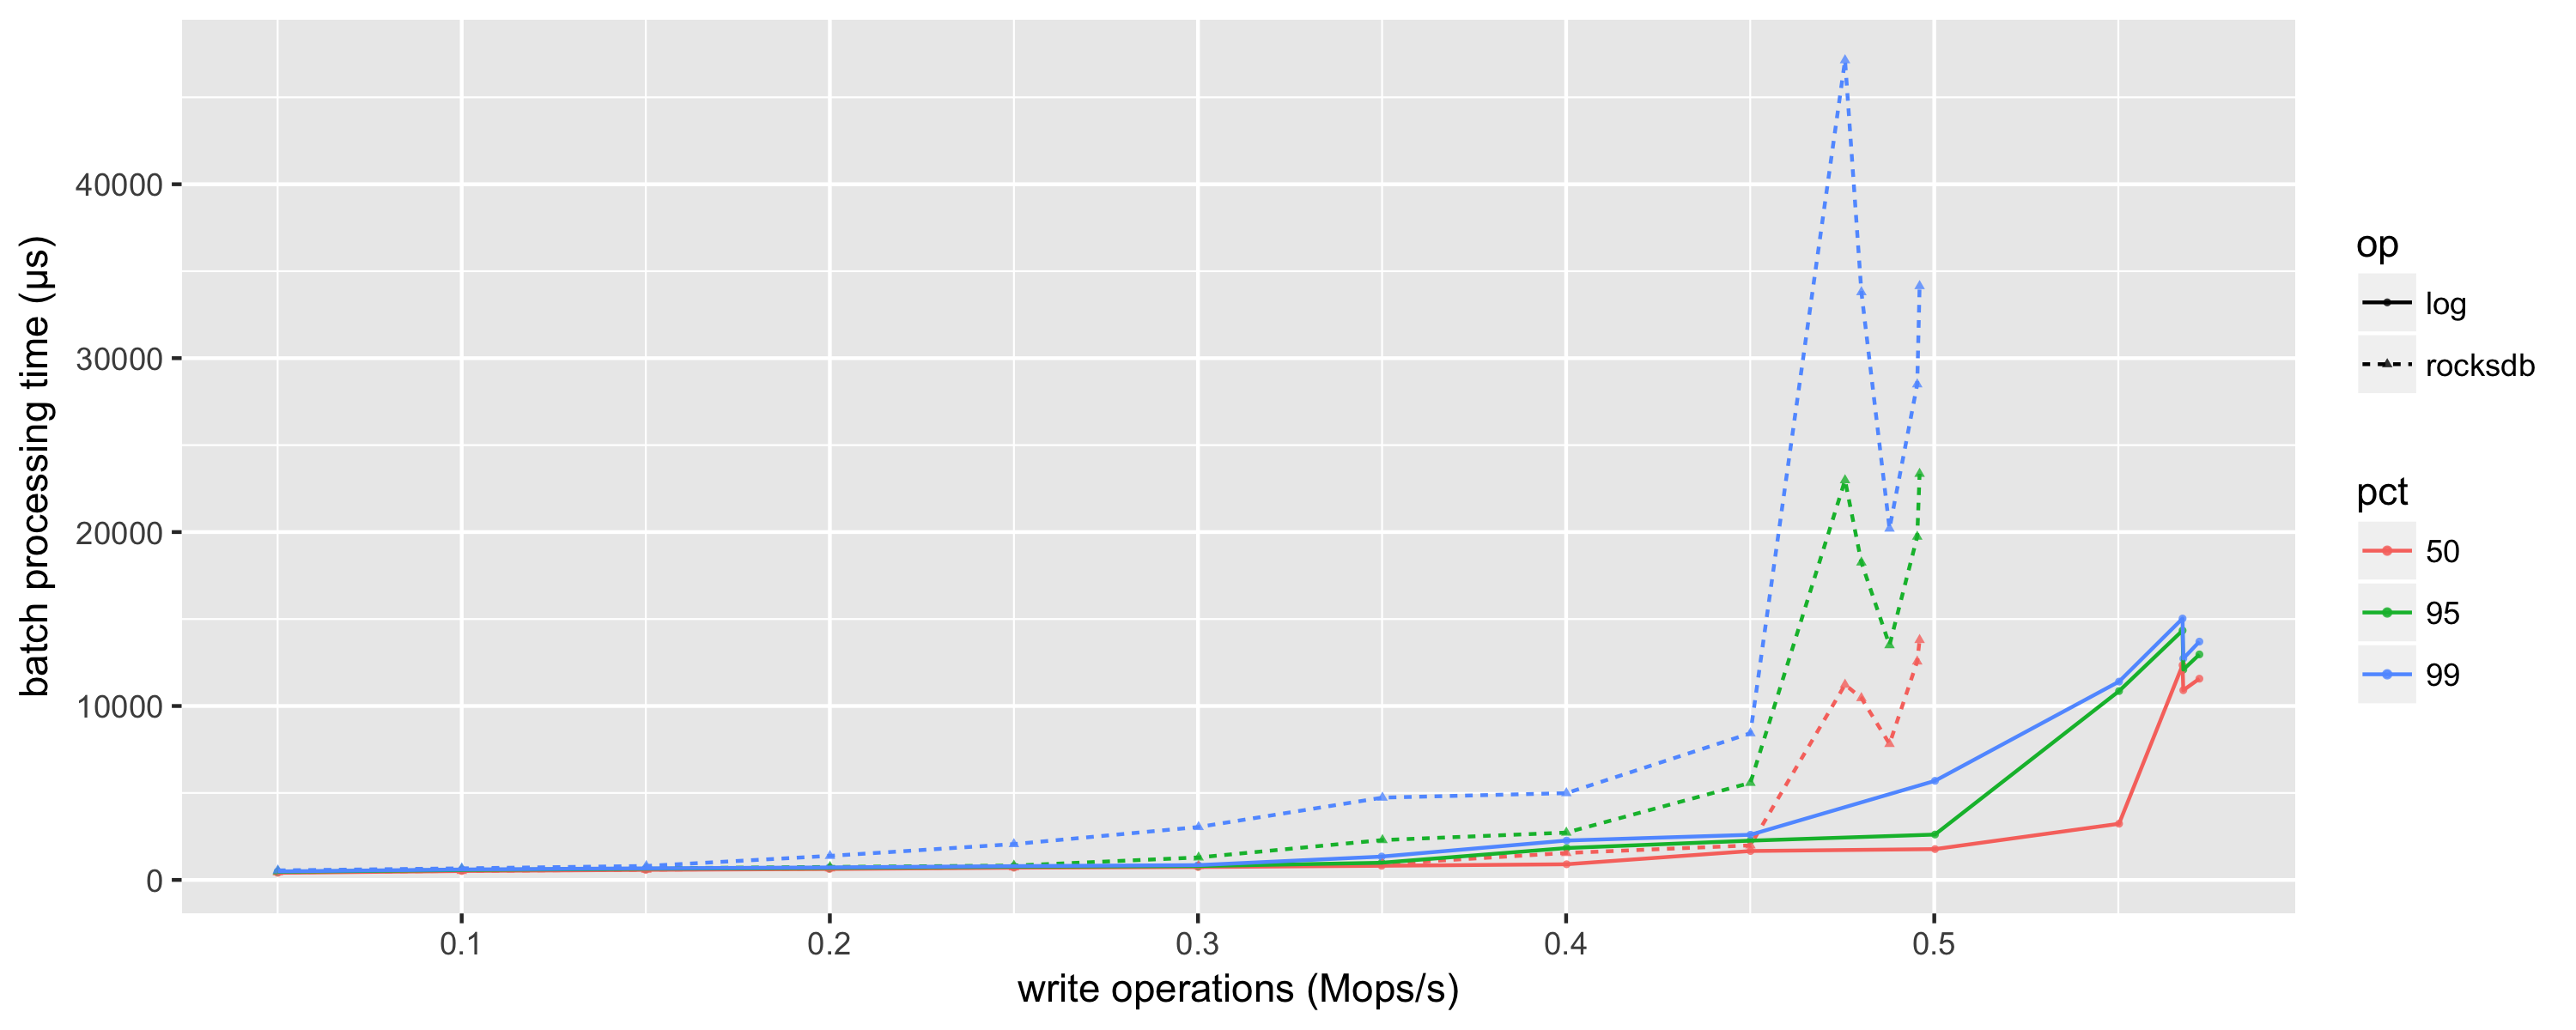
\includegraphics[width=\textwidth]{graphs/write-batch}
  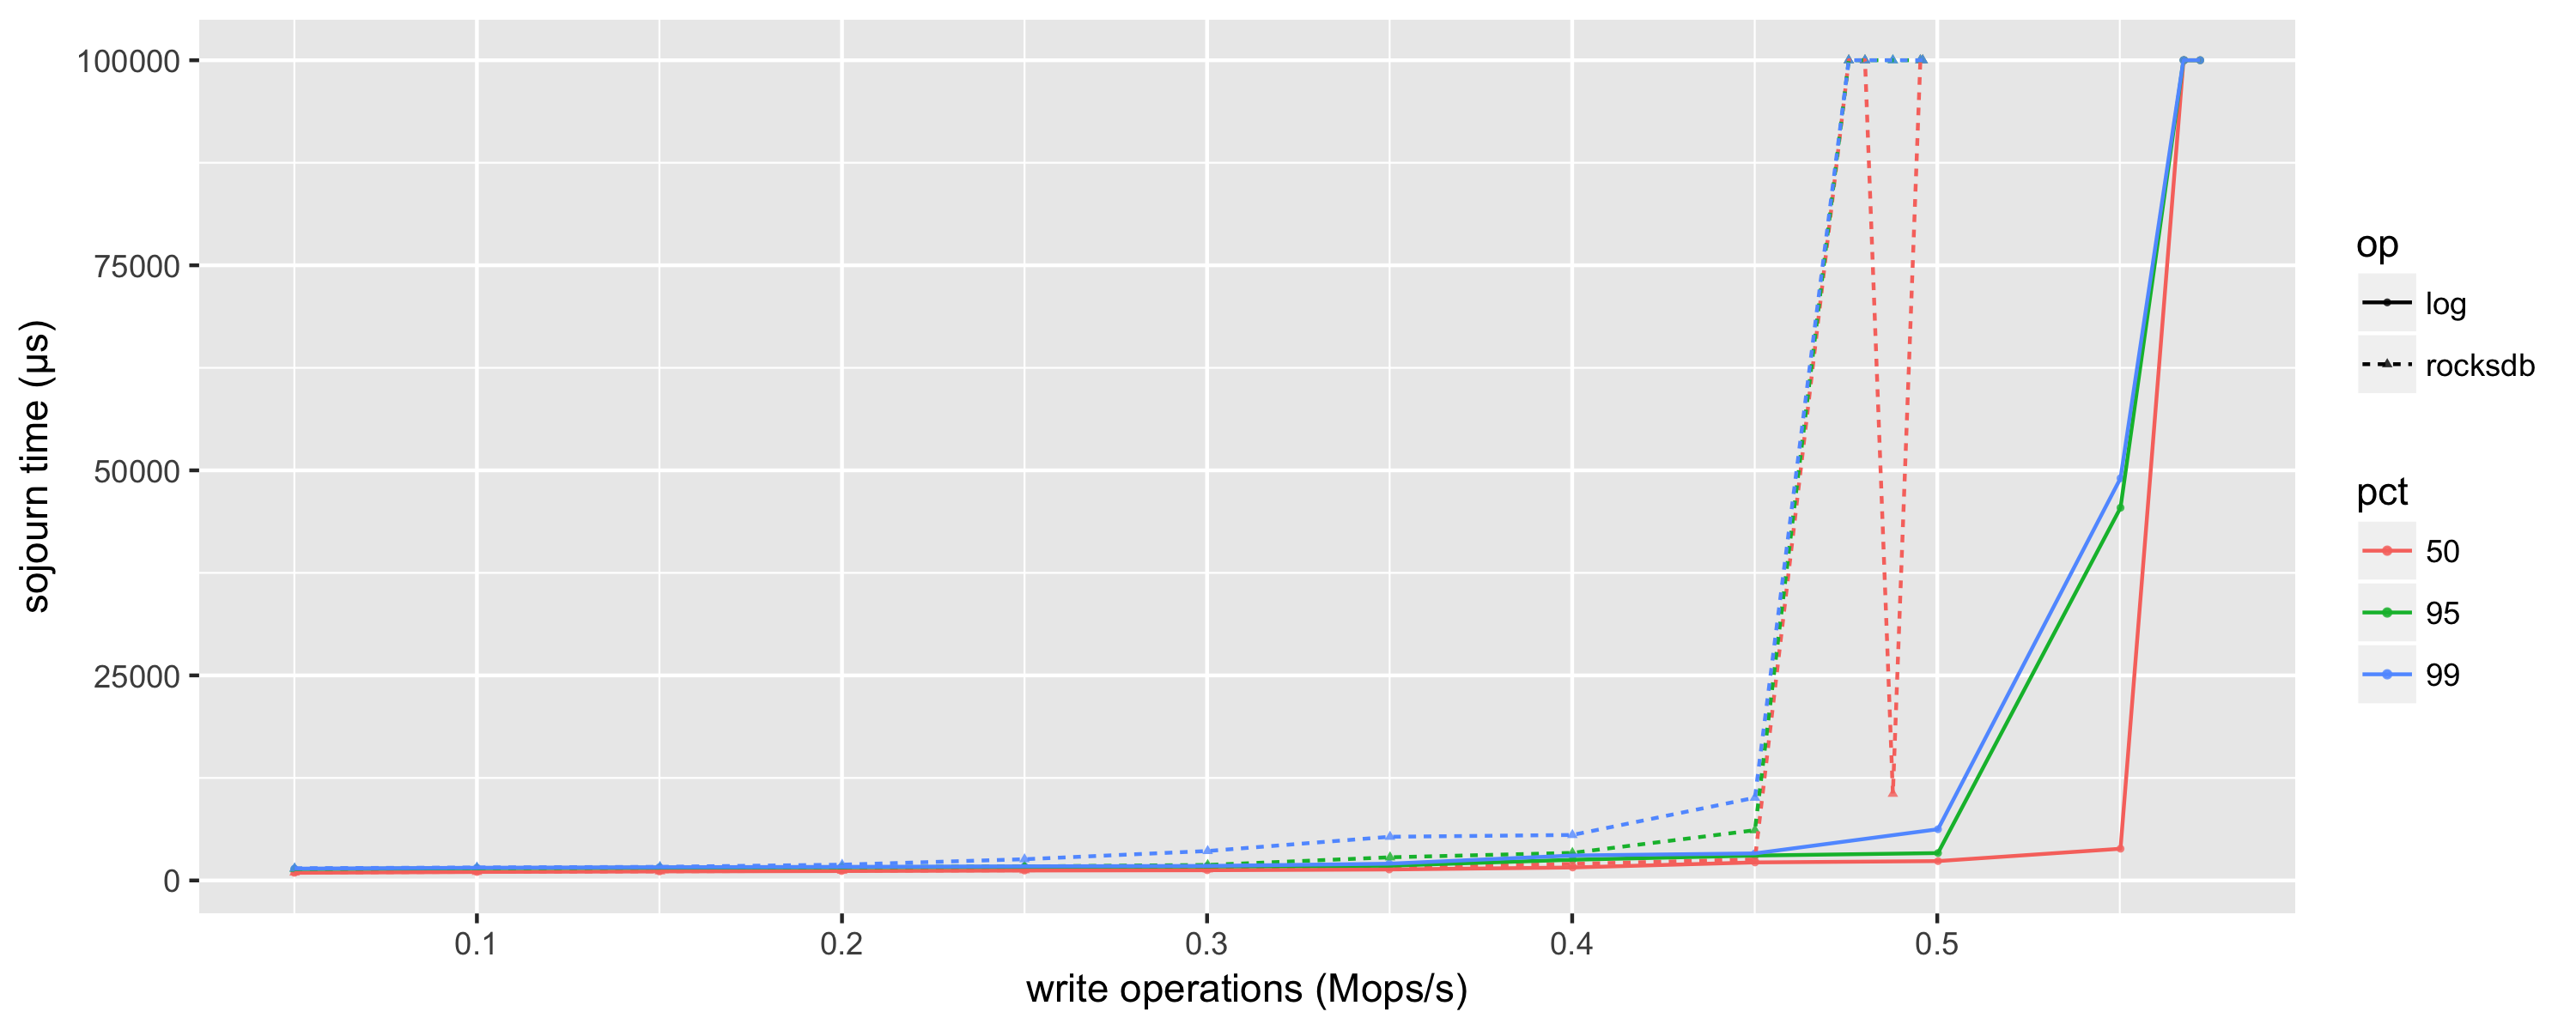
\includegraphics[width=\textwidth]{graphs/write-sjrn}
  \caption{\
    Write-only comparison of Soup's regular write-ahead log and RocksDB.\@ The
    topmost figure shows the latency from when the request was initiated, while
    the bottommost includes the time from the request was generated by the
    open-loop benchmark (see section~\ref{sec:vote-open-loop}).
  }\label{fig:graph-write}
\end{figure}

Materializing base node state to durable storage introduces a slight
write-latency penalty under load. This eventually translates to about a 10\%
decrease in maximum write-throughput, compared to the naive Soup log. Even
though the RocksDB write-ahead log is written to a different disk than its
SS-tables, the amount of data that has to be written to the RocksDB WAL with
\code{PersistentState} is still multiples more than with the Soup log. The
former has to include entries for every index a base node maintains, while the
latter only needs one entry for the update itself.

Additionally, writing to RocksDB's in-memory buffers is not a negligible cost,
especially considering serialization. Whereas the Soup log only needed to
serialize the update once, \code{PersistentState} needs to do so, in-part, once
for each index.

\todo{show a graph comparing memtable implementation speed?}

\section{Read-performance}

When measuring the overall read-performance of Soup as a system, a read heavy
\code{vote} benchmark is a good indicator. To analyze the impact of persisting
state to durable storage at the base nodes we want to ensure that we are
actually measuring the read performance of the \textit{base nodes} however, and
not the partial nodes further down the graph. Instead, we will make use of the
replay benchmark described in section~\ref{sec:bench-replay}, where each row is
read at most once, resulting in a full replay from the base nodes.

The database is pre-populated with 10 million rows, after which a small random
subset of the rows are read once. With \code{PersistentState}, Soup recovers
existing data between each test run, after flushing the disk caches.

\begin{figure}[H]
  \centering
  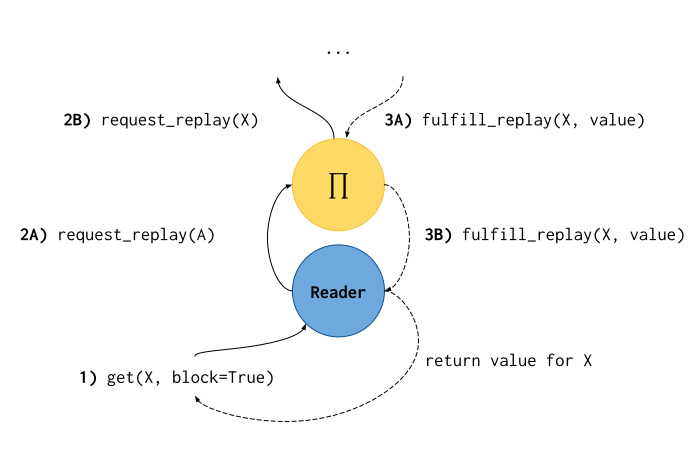
\includegraphics[width=\textwidth]{graphs/replay}
  \caption{\
    The replay performance of in-memory Soup compared to Soup with RocksDB.\@
  }\label{fig:graph-replay}
\end{figure}

\subsection{SS-table format}

RocksDB provides two separate SS-table implementations, \code{BlockBasedTable}
and \code{PlainTable}.

\todo{write more!}

\begin{figure}[H]
  \centering
  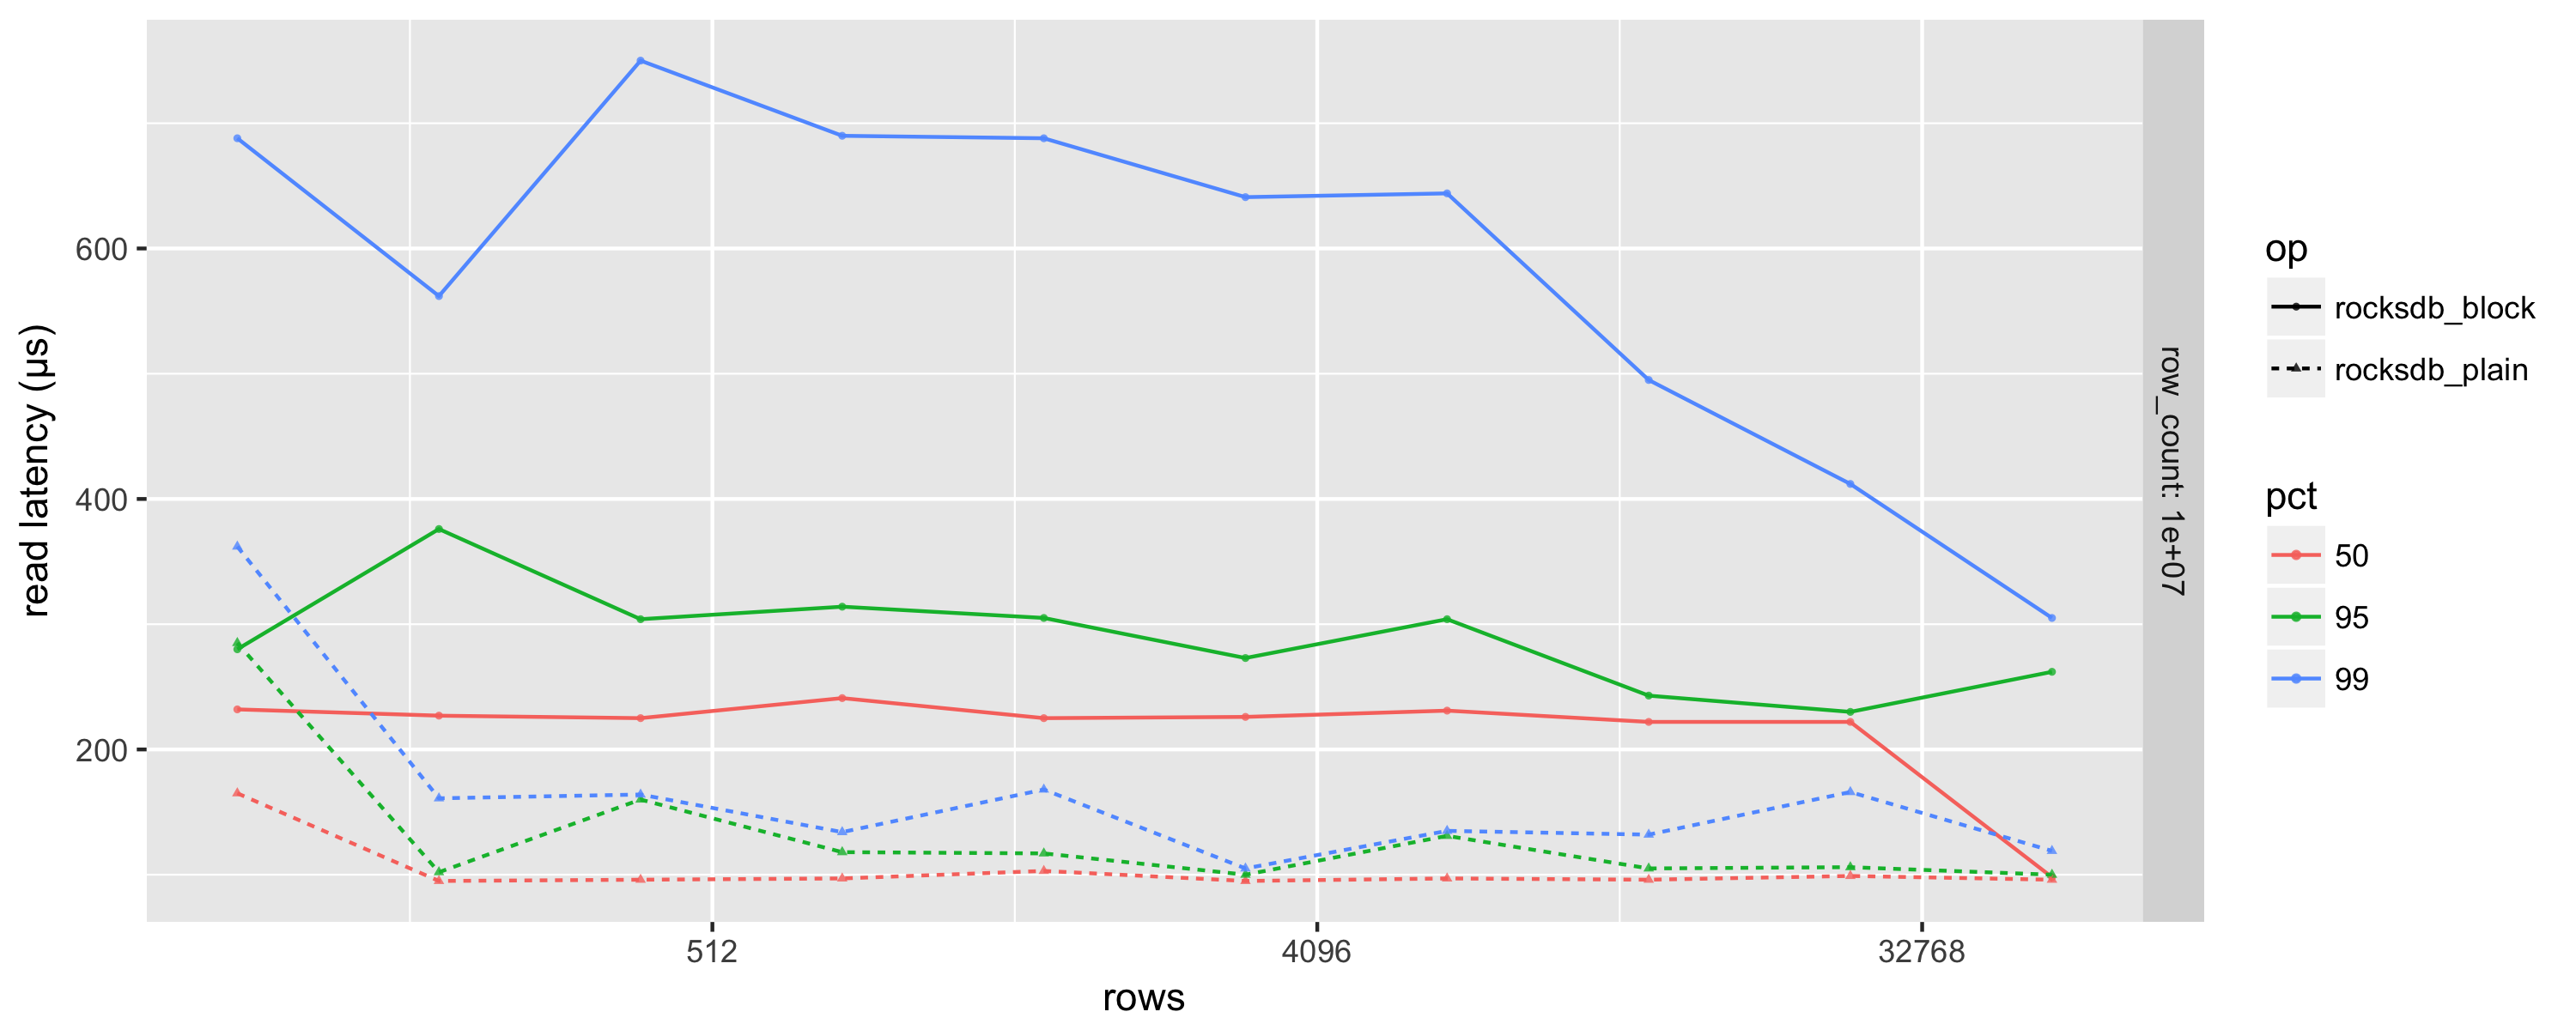
\includegraphics[width=\textwidth]{graphs/replay-table}
  \caption{\
    Soup replay performance comparison between \code{BlockBasedTable} and
    \code{PlainTable}.
  }\label{fig:graph-replay-table}
\end{figure}

\section{Mixed workload}

\section{Recovery}

The recovery benchmark introduced in section~\ref{sec:bench-recovery} helps us
compare the impact different durability strategies have on the time it takes to
recover after a failure. For every data point, the database is populated with
10K articles and a varying amount of votes divided evenly between the articles.
After population, Soup is restarted, while the time it takes to recover is
measured. The state is considered recovered when the total sum of votes returned from
reading all articles equal the actual amount of votes in the system---signified
as \textit{total} in figure~\ref{fig:graph-recovery}.

Unlike the other durability methods, recovering with durable base nodes does not
affect the partial nodes further down the graph---they remain empty until future
read operations trigger ancestor queries to the base nodes. Snapshotting, on the
other hand, brings all materialized nodes in the graph back to the state they
were in prior to crashing. This is the case for log-recovery as well, as updates
from the WAL propagate through the entire graph when recovering. To highlight
this divide, the time it takes to read a single key after recovering from a
durable base node application is measured as well, denoted as \textit{initial}
in figure~\ref{fig:graph-recovery}.

\begin{figure}[H]
  \centering
  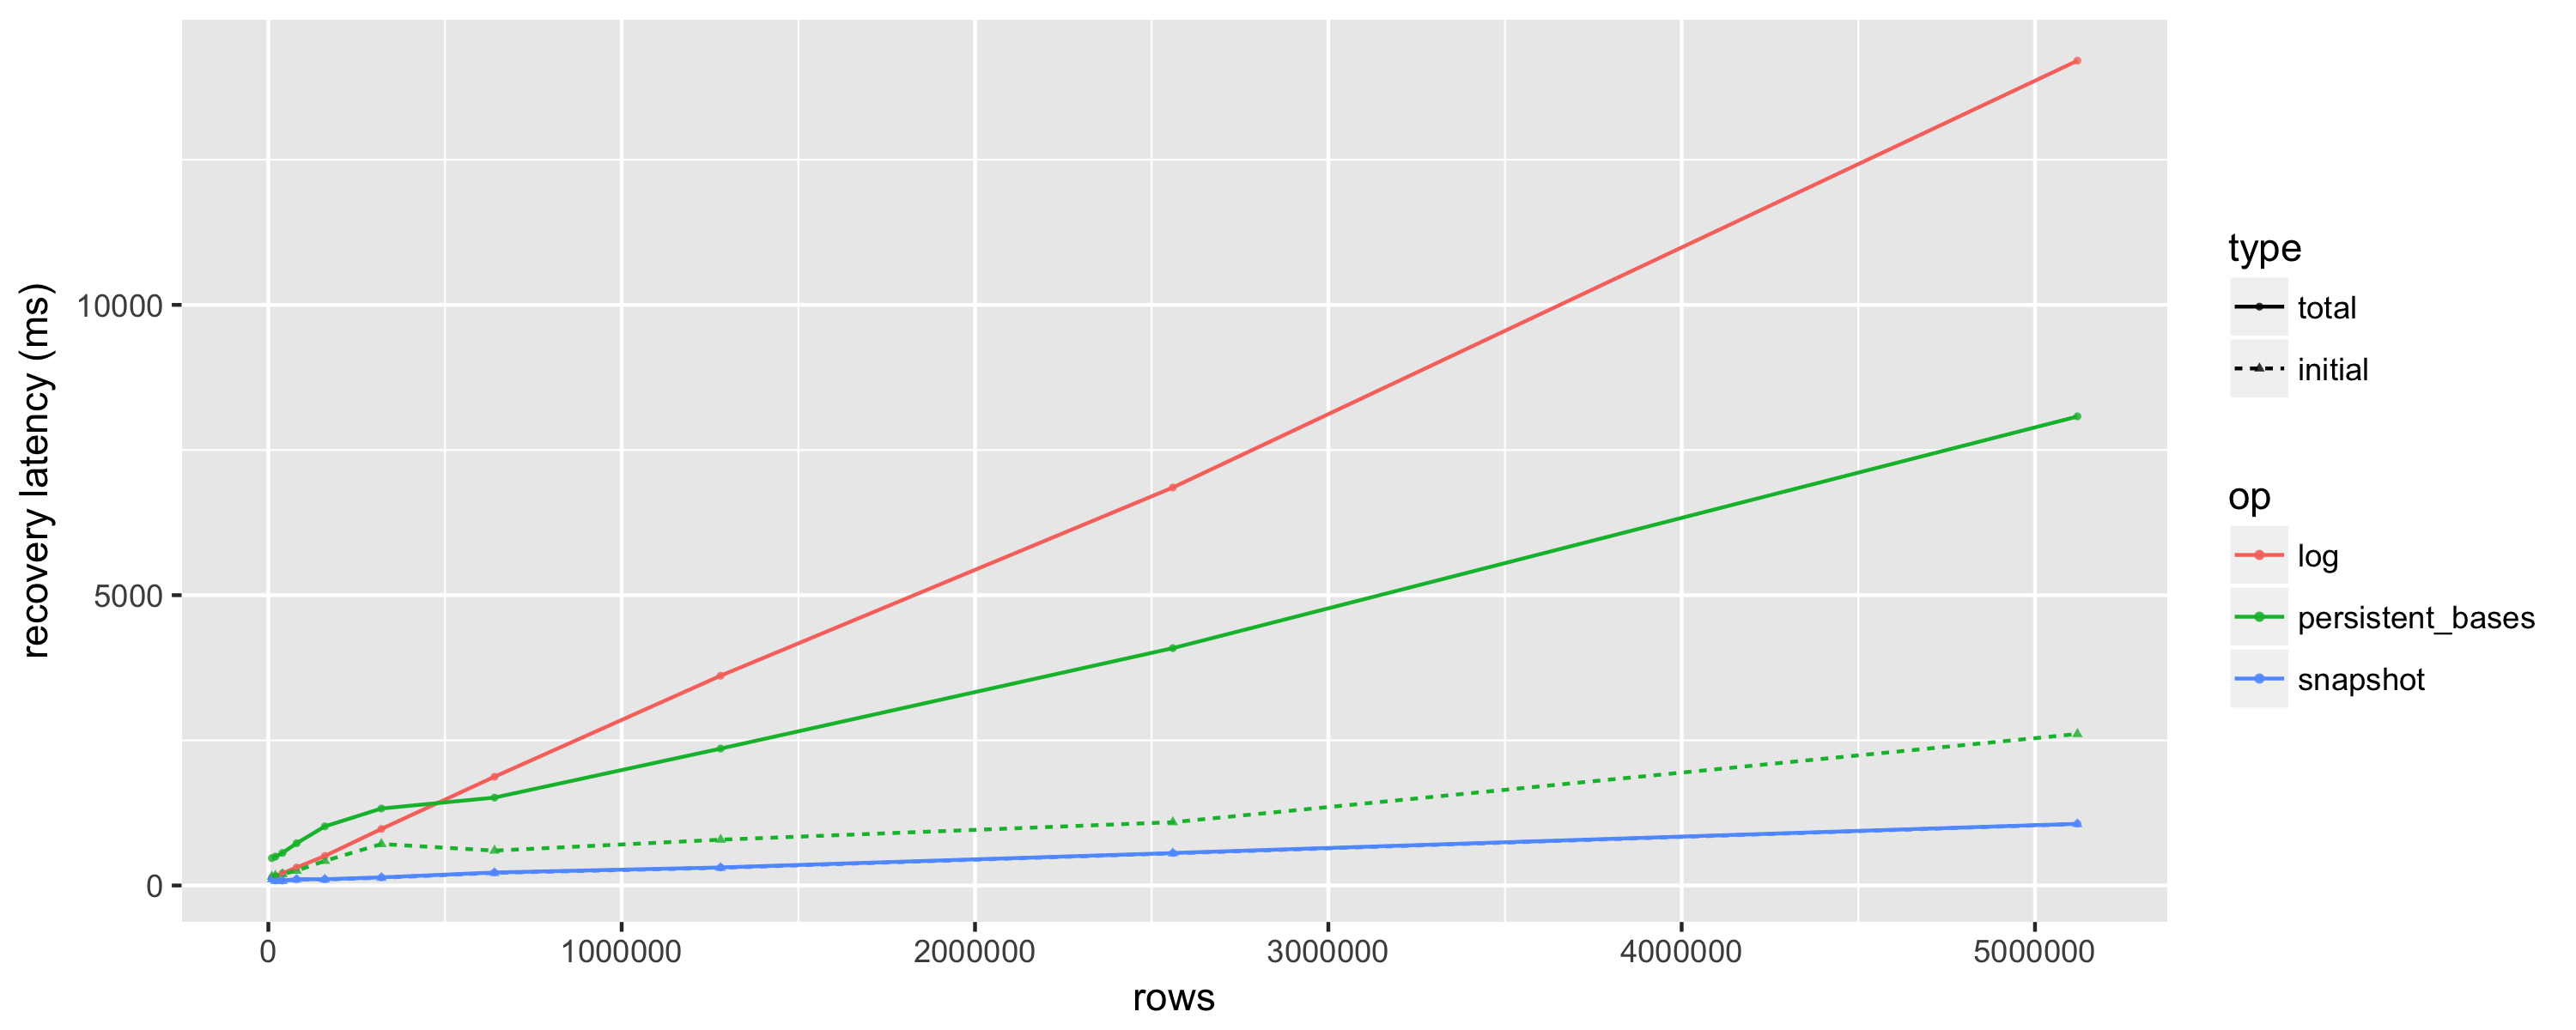
\includegraphics[width=\textwidth]{graphs/recovery}
  \caption{\
    The recovery benchmark measures the time it takes to recover after
    a failure. The \textit{initial} metric highlights the latency of reading a
    single key, while \textit{total} requires all reads to return the same
    result as prior to crashing.
  }\label{fig:graph-recovery}
\end{figure}

The results are pretty much as expected. Snapshotting returns all the
materialized nodes in the graph to their correct state, avoiding the need to
replay any state after recovering. The time it takes to recover still increases
after a while, with more data to read from disk. Log-based recovery needs to go
through \textit{all} updates since the beginning of time before it is considered
ready, resulting in poor performance. With durable base nodes, each read
requires a full replay from the bases---a significant latency penalty when the
row count goes up.

With \code{PersistentState}, the base nodes do not have to process any updates
at all when recovering. Restoring \code{PersistentState} to the correct state is
left to RocksDB, which puts a cap on recovery time by ensuring that its
write-ahead logs never grow beyond a given size. Recovering the actual database
files, the SS-tables, is ``free''---no data needs to be read into memory.

\subsection{Compressing Snapshots}

\todo{re-run benchmarks with compression}

\subsection{Write-performance with Snapshotting}

Snapshotting is a significant improvement to Soup's recovery situation, and a
step in the right direction for Soup as a production-ready system. Regardless,
it is only useful if Soup manages to maintain much of the same write-throughput
while performing regular snapshots.

To measure the performance penalty of snapshotting, we make use of the vote
benchmark described in section~\ref{sec:vote} and earlier in this chapter. The
benchmark compares the batch write latency at increasing throughput targets,
first without snapshotting and then with. The benchmark runs for 60 seconds,
performing a snapshot every 10 seconds.

\begin{figure}[H]
  \centering
  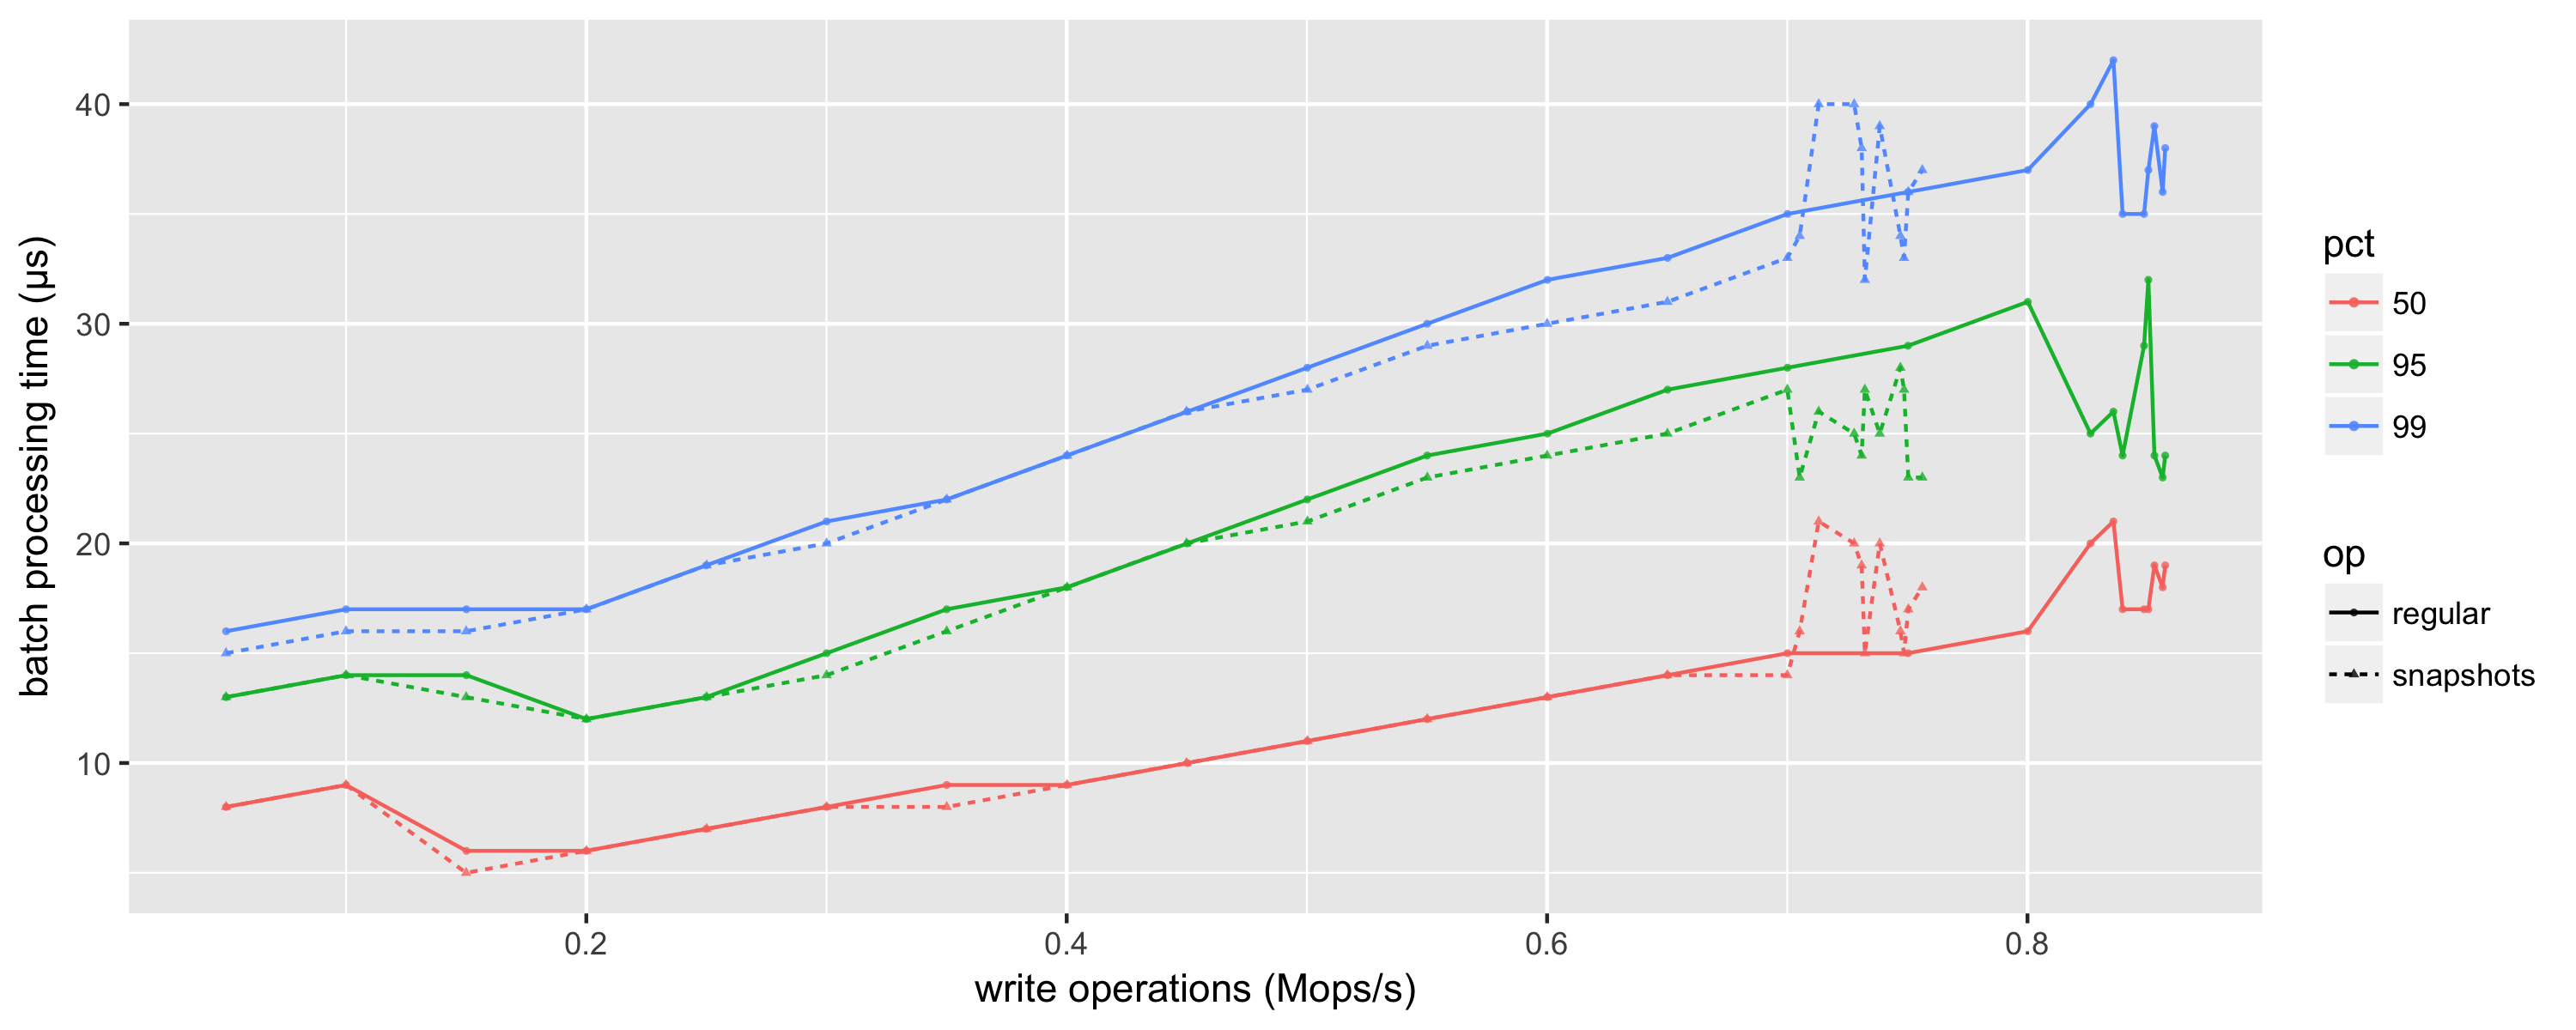
\includegraphics[width=\textwidth]{graphs/write-snapshot-batch}
  \caption{\
    Write-latency comparison with and without snapshotting (with a snapshot
    timeout of 10 seconds). Both use Soup's regular write-ahead log.
  }\label{fig:graph-snapshot}
\end{figure}

Most of the snapshotting work is performed in standalone snapshot workers,
running in threads separate from Soup's packet processing. Without this, the
throughput penalty would without doubt be much more significant than the 10\%
observed in figure~\ref{fig:graph-snapshot}. The penalty is a result of the full
state clone incurred at each materialized node during a snapshot.

\begin{figure}[H]
  \centering
  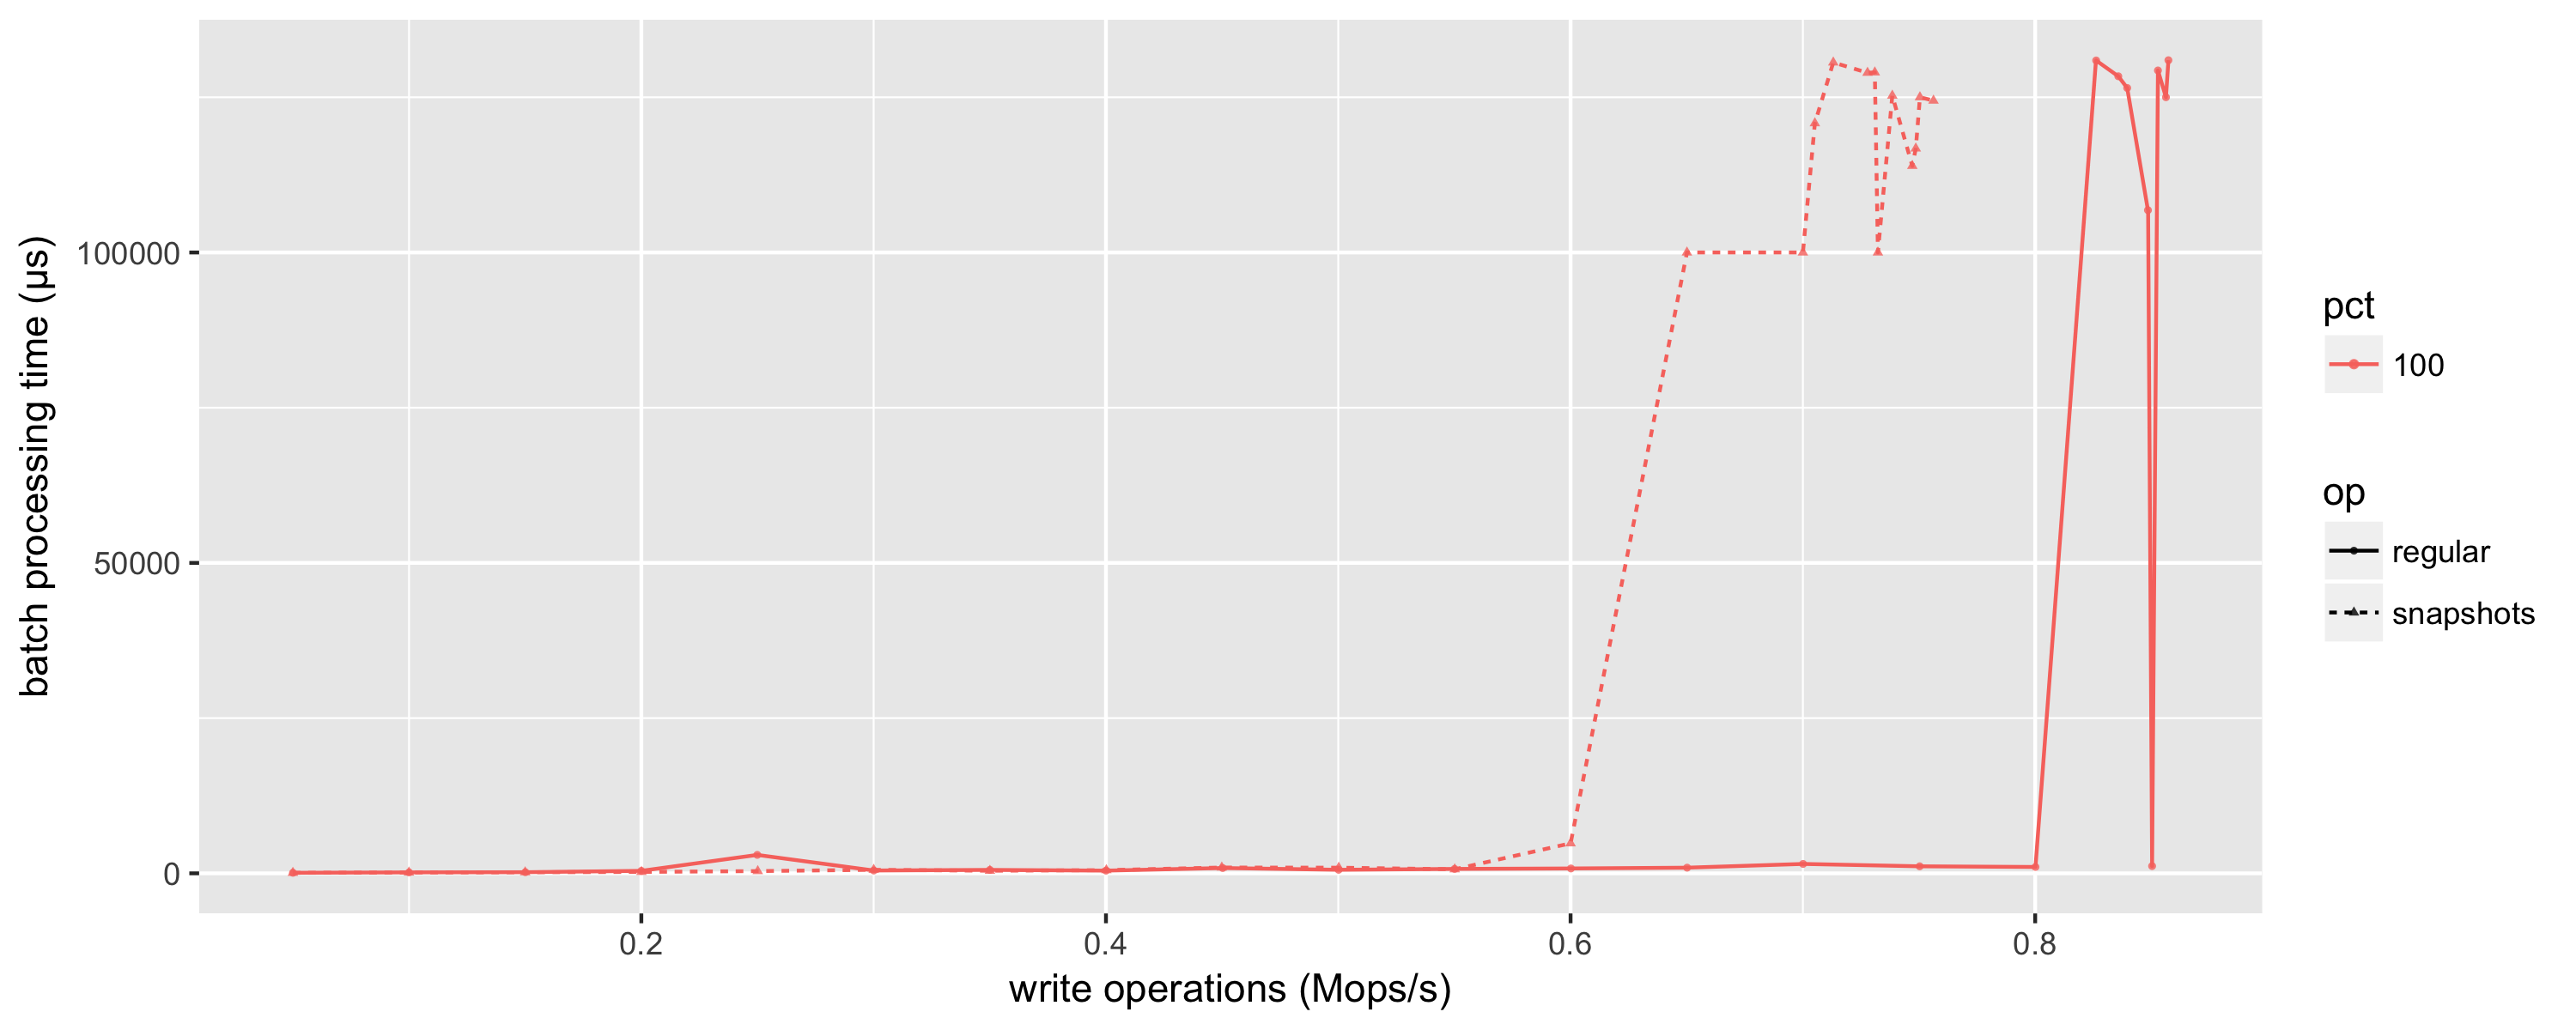
\includegraphics[width=\textwidth]{graphs/write-snapshot-100-batch}
  \caption{\
    100th percentile comparison, with and without snapshotting.
  }\label{fig:graph-snapshot-100}
\end{figure}

The first snapshot graph shows no increase in latency. With a snapshot timeout
of 10 seconds and a benchmark runtime of 60 seconds, snapshot occurrences are
probably too rare for it to show up in the 95th percentile. Looking at the 100th
percentile on the other hand, we can see the latency spiking at a lower
throughput than normal. At this point the state size is reasonably large,
resulting in non-trivial clone operations.
